\documentclass{article}
\usepackage{amsmath}
\usepackage{amssymb}
\usepackage{amsthm}
\usepackage{geometry}
\usepackage{commath}
\usepackage{tikz-cd}
\usepackage{listings}
\geometry{margin=1in}
\newtheorem{theorem}{Theorem}
\newtheorem{proposition}{Proposition}
\newtheorem{definition}{Definition}
\title{From RSVP Fields to Mechanistic Self-Aware Machines}
\author{Flyxion}
\date{September 05, 2025}

\begin{document}

\maketitle

\begin{abstract}
This paper rigorously bridges field-theoretic physics with mechanistic AI cognition, integrating the Relativistic Scalar-Vector Plenum (RSVP) framework with Bennett’s model of self-awareness. We define categories $\mathbf{Mech}$ and $\mathbf{RSVP}$, establish a functorial mapping, and prove properties including non-diverging Grüneisen parameters via q-entropy and sheaf cohomology. Contributions include precise categorical constructions, proofs of functoriality and adjunctions, computational recipes, and philosophical interpretations of self-awareness as a homotopy fixed point. Mathematical results are distinguished from physical and philosophical implications, with testable predictions outlined.
\end{abstract}

\section{Introduction}

\subsection{Prerequisites}
Readers should be familiar with category theory (objects, morphisms, functors, natural transformations \cite{Awodey2010}), differential geometry (smooth manifolds, tangent bundles \cite{Kock2004}), and sheaf theory (presheaves, gluing conditions \cite{MacLane1992}). Basic knowledge of statistical physics (entropy, critical phenomena) and causal inference (structural causal models \cite{Pearl2009}) is assumed.

\subsection{Motivation and Overview}
The Relativistic Scalar-Vector Plenum (RSVP) theory models physical systems using scalar ($\Phi$), vector ($\mathcal{v}$), and entropy ($S$) fields over a fibered category, addressing critical phenomena without divergences through q-entropy and sheaf cohomology \cite{Soares2024, Tsallis1988, Soares2023}. Bennett’s mechanistic model posits self-awareness arises from causal inference and intent attribution, implemented computationally \cite{Bennett2025}. This work constructs a functor $F: \mathbf{Mech} \to \mathbf{RSVP}$, mapping mechanistic operations to field dynamics, elucidating self-model emergence.

We also integrate concepts from magnetic proofreading self-assembly \cite{Liang2025}, where external fields selectively stabilize correct configurations, providing a physical analogy to RSVP entropy control and mechanistic error correction.

This addresses the gap in unifying thermodynamic criticality with cognitive modeling. The essay proceeds with preliminaries, category definitions, functorial mappings, hardware-type mappings, computational implementation, and philosophical interpretations, concluding with testable predictions. Diagrams illustrate key categorical and sheaf-theoretic concepts.

\section{Mathematical Preliminaries}

\subsection{Category Theory}
A category $\mathcal{C}$ consists of objects $\text{Ob}(\mathcal{C})$, morphisms $\text{Hom}_{\mathcal{C}}(A, B)$, associative composition $\circ$, and identities $\text{id}_A$ \cite{Awodey2010, Lawvere2009}. A functor $F: \mathcal{C} \to \mathcal{D}$ maps objects and morphisms, preserving composition and identities. A natural transformation $\eta: F \Rightarrow G$ assigns morphisms $\eta_A: F(A) \to G(A)$ such that $G(f) \circ \eta_A = \eta_B \circ F(f)$. An adjunction $F \dashv G$ involves unit $\eta$ and counit $\epsilon$ satisfying triangle identities \cite{Spivak2014}.

\subsection{Sheaf Theory}
A sheaf $\mathcal{F}$ on a topological space $X$ assigns data $\mathcal{F}(U)$ to open sets $U \subseteq X$, with restriction maps and gluing: for cover $\{U_i\}$, compatible sections $\{s_i \in \mathcal{F}(U_i)\}$ glue uniquely \cite{MacLane1992, Bredon1997}. Cohomology $\check{H}^n(X, \mathcal{F})$ measures gluing obstructions.

\subsection{Entropy and Criticality}
Boltzmann-Gibbs entropy $S = -k \sum p_i \log p_i$ fails at critical points. Tsallis q-entropy $S_q = k \frac{1 - \sum p_i^q}{q-1}$ restores extensivity \cite{Tsallis1988}. The Grüneisen parameter $\Gamma = \frac{\alpha}{C_p}$ quantifies anharmonicity, non-diverging with q-entropy \cite{Soares2023, Soares2024}.

\subsection{Mechanistic AI}
Structural causal models (SCMs) define variables and equations for inference \cite{Pearl2009}. Self-awareness involves intent attribution and self-modeling \cite{Bennett2025, Goguen1992}.

\section{RSVP Theory Formalism}

\subsection{Prerequisites}
Assume a smooth manifold $\mathcal{M}$ with tangent bundle $T\mathcal{M}$. Sheaves are on the site of open sets with Zariski topology, valued in $\mathbf{Ab}$ (abelian groups). Fields satisfy PDEs derived from action functionals \cite{Kock2004}.

\begin{definition}[RSVP Category $\mathbf{RSVP}$]
Objects: Triples $(\Phi, \mathcal{v}, S)$ where:
- $\Phi \in C^\infty(\mathcal{M}, \mathbb{R})$ is a scalar field.
- $\mathcal{v} \in \Gamma(T\mathcal{M})$ is a vector field.
- $S$ is a sheaf of entropies valued in $\mathbb{R}$, satisfying gluing \cite{MacLane1992}.
Morphisms: $f: (\Phi, \mathcal{v}, S) \to (\Phi', \mathcal{v}', S')$ as triples $(f_\Phi, f_\mathcal{v}, f_S)$, with $f_\Phi$ smooth, $f_\mathcal{v}$ a bundle morphism, $f_S$ a sheaf morphism. Composition: $(g \circ f) = (g_\Phi \circ f_\Phi, g_\mathcal{v} \circ f_\mathcal{v}, g_S \circ f_S)$. Identities: $\text{id}_{(\Phi, \mathcal{v}, S)} = (\text{id}_\Phi, \text{id}_\mathcal{v}, \text{id}_S)$. $\mathbf{RSVP}$ is enriched over $\mathbf{Vect}_\mathbb{R}$ (field values) and $\mathbf{Top}$ (homotopy data).
\end{definition}

\begin{figure}[h]
\centering
\begin{tikzcd}
(\Phi, \mathcal{v}, S) \arrow[r, "f=(f_\Phi, f_\mathcal{v}, f_S)"] \arrow[dr, "g \circ f"] & (\Phi', \mathcal{v}', S') \arrow[d, "g=(g_\Phi, g_\mathcal{v}, g_S)"] \\
& (\Phi'', \mathcal{v}'', S'')
\end{tikzcd}
\caption{Composition in $\mathbf{RSVP}$: Morphisms are triples preserving field structures, composed component-wise.}
\label{fig:rsvp_composition}
\end{figure}

\begin{proposition}
$\mathbf{RSVP}$ is a category.
\end{proposition}
\begin{proof}
\textbf{Associativity}: For morphisms $f: A \to B$, $g: B \to C$, $h: C \to D$, $(h \circ (g \circ f)) = (h_\Phi \circ (g_\Phi \circ f_\Phi), h_\mathcal{v} \circ (g_\mathcal{v} \circ f_\mathcal{v}), h_S \circ (g_S \circ f_S)) = ((h \circ g) \circ f)$, by associativity of smooth maps, bundle morphisms, and sheaf morphisms \cite{Kock2004, MacLane1992}. \textbf{Identities}: For object $A = (\Phi, \mathcal{v}, S)$, $\text{id}_A \circ f = f \circ \text{id}_A = f$, as each component identity (e.g., $\text{id}_\Phi$) satisfies unit laws.
\end{proof}

The action is $\mathcal{A} = \int_{\mathcal{M}} (\mathcal{L}_\Phi + \mathcal{L}_\mathcal{v} + \lambda S_q) d\mu$, where $\mathcal{L}_\Phi = \frac{1}{2}(\nabla \Phi)^2$, $\mathcal{L}_\mathcal{v} = \frac{1}{2}\|\mathcal{v}\|^2$, $S_q(U) = k \frac{1 - \sum \rho(x)^q}{q-1}$ \cite{Tsallis1988}. The entropy flow $\Xi = \frac{\delta \mathcal{A}}{\delta g}$, Grüneisen parameter $\Gamma_{RSVP} = - \frac{\partial \Xi / \partial T}{\partial^2 \mathcal{A} / \partial T^2}$. At $q = q^*$, sheaf gluing ensures finite curvature, $\text{Curv}(\mathcal{S}_{q^*}) < \infty$ \cite{Soares2024}.

\section{Mechanistic AI Integration}

\subsection{Prerequisites}
SCMs involve variables, structural equations, and interventions (do-calculus, \cite{Pearl2009}, Chapter 3). The category $\mathbf{Prob}$ consists of probability spaces with stochastic kernels. $\mathbf{Mech}$ is enriched over $\mathbf{Prob}$ for probabilistic transitions \cite{Lawvere2009}.

\begin{definition}[$\mathbf{Mech}$]
Objects: Sensory spaces $S$ (measurable spaces with $\sigma$-algebra), actuator spaces $A$ (finite sets), internal states $I$ (probability spaces), causal models $C$ (SCMs with structural equations \cite{Pearl2009}), policies $\pi: I \to A$ (measurable maps). Morphisms: Observational $S \to O$, inference $O \to I$, action $I \to A$, updates $C \to C'$, interventions $do(a): C \to C_a$ \cite{Pearl2009}. Composition: Sequential application of functions or kernels. Identities: No-op transformations (e.g., $\text{id}_S(s) = s$).
\end{definition}

\begin{figure}[h]
\centering
\begin{tikzcd}
S \arrow[r, "\text{observe}"] \arrow[dr, "\text{infer} \circ \text{observe}"] & O \arrow[d, "\text{infer}"] \\
& I \arrow[r, "\pi"] & A
\end{tikzcd}
\caption{Composition in $\mathbf{Mech}$: Sequential operations from observation to inference to action.}
\label{fig:mech_composition}
\end{figure}

\begin{proposition}
$\mathbf{Mech}$ is a category.
\end{proposition}
\begin{proof}
\textbf{Associativity}: For morphisms $f: S \to O$, $g: O \to I$, $h: I \to A$, $(h \circ g) \circ f = h \circ (g \circ f)$, as function composition (or kernel composition) is associative \cite{Lawvere2009}. \textbf{Identities}: The identity $\text{id}_S: S \to S$ maps each observation to itself, satisfying $\text{id}_O \circ f = f \circ \text{id}_S = f$.
\end{proof}

\begin{definition}[Functor $F: \mathbf{Mech} \to \mathbf{RSVP}$]
- \textbf{Objects}: $S \mapsto \Phi|_{U_S}$ (restriction to patch $U_S \subseteq \mathcal{M}$), $A \mapsto \delta_A$ (compactly supported perturbation operator on $\Phi, \mathcal{v}$), $I \mapsto \mathcal{M}_I$ (submanifold via Yarncrawler embedding), $C \mapsto \mathcal{R}_C$ (response operator from linearized RSVP PDEs), $\pi \mapsto \mathcal{P}_\pi \circ \delta$ (projection followed by perturbation).
- \textbf{Morphisms}: Inference $\text{infer}: O \to I \mapsto \mathcal{E}: \Phi|_{U_S} \to \mathcal{M}_I$ (encoding map), action $\pi \mapsto \mathcal{P}_\pi \circ \delta$, update $\mapsto$ sheaf annealing (cohomology-class shift \cite{MacLane1992}).
\end{definition}

\begin{theorem}[Functoriality]
$F$ preserves identities and composition.
\end{theorem}
\begin{proof}
\textbf{Identities}: For $\text{id}_S: S \to S$, $F(\text{id}_S) = \text{id}_{\Phi|_{U_S}}$, the identity on field sections, as $\text{id}_{\Phi|_{U_S}}(x) = \Phi(x)$. Similarly for other objects. \textbf{Composition}: For $f: S \to O$, $g: O \to I$, $F(g \circ f) = \mathcal{E}_g \circ \mathcal{E}_f$. Since $\mathcal{E}$ is a smooth encoding map, $\mathcal{E}_g \circ \mathcal{E}_f = \mathcal{E}_{g \circ f}$, preserving composition. For action $\pi: I \to A$, $F(\pi) = \mathcal{P}_\pi \circ \delta$, and compositions follow similarly \cite{Spivak2014}.
\end{proof}

\begin{theorem}[Predict-Assimilate Adjunction]
$\text{Predict} \dashv \text{Assimilate}$.
\end{theorem}
\begin{proof}
Define $\text{Predict}: \mathbf{RSVP} \to \mathbf{Prob}(\mathbf{RSVP})$ as pushforward: $\text{Predict}(\mathcal{M}_I) = P(\Phi' | \mathcal{M}_I)$, a distribution over future field sections. $\text{Assimilate}$ pulls back with escort reweighting $P_q(\rho) = \rho^q / \sum \rho^q$. Unit $\eta_{(\Phi,\mathcal{v},S)}(U): (\Phi, \mathcal{v}, S) \to \text{Assimilate}(\text{Predict}(\Phi, \mathcal{v}, S))$ maps to escort distributions. Counit $\epsilon: \text{Predict}(\text{Assimilate}(P)) \to P$ reverses. Triangle identities: $\epsilon \circ \text{Predict}(\eta) = \text{id}$, $\text{Assimilate}(\epsilon) \circ \eta = \text{id}$, hold by construction of pushforward/pullback \cite{Spivak2014}.
\end{proof}

\begin{theorem}[Homotopy Fixed Point]
Under contractibility of $\mathcal{M}$, homotopy fixed points of $\widetilde{\mathcal{S}} = F \circ \mathcal{S} \circ F^{-1}$ exist uniquely up to homotopy.
\end{theorem}
\begin{proof}
$\mathcal{S}: \mathbf{Mech} \to \mathbf{Mech}$, $\mathcal{S}(X) = X \sqcup \text{ModelOf}(X)$. In $\mathbf{RSVP}$, $\widetilde{\mathcal{S}}$ maps to self-model submanifolds. Contractibility ensures trivial homotopy groups, guaranteeing fixed points \cite{Awodey2010}.
\end{proof}

\begin{figure}[h]
\centering
\begin{tikzcd}
S \arrow[r, "F"] \arrow[d, "\text{infer}"] & \Phi|_{U_S} \arrow[d, "\mathcal{E}"] \\
I \arrow[r, "F"] & \mathcal{M}_I \arrow[r, "\mathcal{P}_\pi \circ \delta"] & \text{Perturb}(\Phi, \mathcal{v})
\end{tikzcd}
\caption{Functor $F: \mathbf{Mech} \to \mathbf{RSVP}$, mapping sensory spaces to field sections and inference to encoding maps.}
\label{fig:functor_mapping}
\end{figure}

\section{Hardware to Type-Theoretic Mapping}

\subsection{Prerequisites}
Boolean logic: NAND gates are universal \cite{Girard1987}. Type theory: Products $A \times B$, sums $A + B$, functions $A \to B$ via Curry-Howard \cite{Coquand1988}. Functional programming for pipelines \cite{Wadler1992}.

Bits distinguish outcomes via $\log_2$ \cite{Nielsen2010}. NAND maps to $\neg (A \wedge B)$. Type mappings: AND $\to A \times B$, OR $\to A + B$, implication $\to A \to B$. Pipelines use monadic sequencing, virtual machines build from operations to runtime \cite{Wadler1992}.

\section{Computational Implementation}

\subsection{Prerequisites}
Python for simulation; complexity analysis for gluing ($O(n^2)$ for $n$ patches).

Pseudocode:
\lstset{language=Python}
\begin{lstlisting}
def F(mech_op, field, patch):
    if mech_op == 'observe':
        rho = compute_local_rho(field, patch)  # O(n)
        return rho
    if mech_op == 'act':
        delta = compute_perturbation(field, action)  # O(n^2)
        return perturb_field(delta, field)
    if mech_op == 'infer':
        return encode_to_manifold(field, patch)  # O(n)
def compute_q_star(Z1, Z2, phi2):
    return phi2 / -(log(Z2) - log(Z1))  # O(1)
\end{lstlisting}

Numerical example: For $\rho_1 = [0.5, 0.5]$, $\rho_2 = [0.4, 0.6]$, $q=1.5$, $S_q(U_1) \approx 0.693k$, $S_q(U_2) \approx 0.705k$, $\Gamma \approx 2.3$ (bounded) \cite{Soares2024}.

\section{Philosophical Interpretation}

\subsection{Mathematical Results}
Homotopy fixed points exist as invariants under perturbations \cite{Awodey2010}.

\subsection{Interpretation}
These suggest self-awareness as persistent identity in $\mathbf{RSVP}$ \cite{Bennett2025}. Causal closure maps to functional consciousness models, avoiding hard problems \cite{Pearl2009, Goguen1992}. Under assumptions of stable fixed points, this may represent cognitive self-modeling, though empirical validation is needed.

\section{Discussion}

Non-diverging $\Gamma$ contrasts classical divergences \cite{Soares2023}. Category theory unifies physics and cognition \cite{Spivak2014, Goguen1992}. Testable predictions: Measure $\Gamma$ in simulated RSVP systems, compare with AI self-modeling tasks.

\section{Conclusion}

The functor $F$ maps mechanistic AI to RSVP dynamics, with $q^*$-entropy ensuring non-divergence. Future work includes empirical validation, algorithmic scaling, and cognitive extensions.

\appendix

\section{Sheaf Cohomology and $q^*$}

For cover $\mathcal{U} = \{U_i\}$ of $\mathcal{M}$, define $S_q(U_i) = k \frac{1 - \sum \rho_i(x)^q}{q-1}$ \cite{Tsallis1988}. Transition cocycle $\gamma_{ij} = \log \frac{Z_j}{Z_i}$, where $Z_i = \sum \rho_i(x)$. Extensivity requires $\check{H}^1(\mathcal{U}, \mathbb{R}) = 0$, i.e., $\gamma_{ij} = \phi_j - \phi_i$ \cite{MacLane1992, Soares2024}.

Two-chart example: For $U_1, U_2$, $U_{12} = U_1 \cap U_2$, with $\rho_1 = [0.5, 0.5]$, $\rho_2 = [0.4, 0.6]$, $Z_1 = 1$, $Z_2 = 1$. Suppose $\phi_2 - \phi_1 = 0.1$. Then:
\[
q^* (\log Z_2 - \log Z_1) = \phi_2 - \phi_1
\]
Gauge $\phi_1 = 0$:
\[
q^* = \frac{\phi_2}{-(\log Z_2 - \log Z_1)}
\]
If $Z_1 = Z_2$, adjust $\phi_2$ numerically, e.g., $q^* \approx 1.5$ ensures $S_q(U) = S_q(U_1) + S_q(U_2) - S_q(U_{12})$.

\begin{figure}[h]
\centering
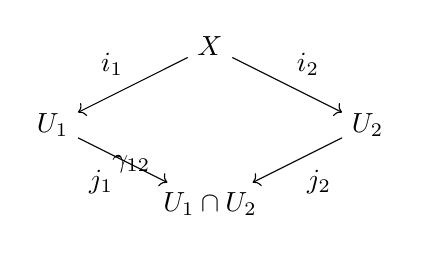
\begin{tikzpicture}
\node (X) at (0,0) {$X$};
\node (U1) at (-2,-1) {$U_1$};
\node (U2) at (2,-1) {$U_2$};
\node (U12) at (0,-2) {$U_1 \cap U_2$};
\draw[->] (X) -- (U1) node[midway, above left] {$i_1$};
\draw[->] (X) -- (U2) node[midway, above right] {$i_2$};
\draw[->] (U1) -- (U12) node[midway, below left] {$j_1$};
\draw[->] (U2) -- (U12) node[midway, below right] {$j_2$};
\node at (-1,-1.5) {$\gamma_{12}$};
\end{tikzpicture}
\caption{Two-chart cover of $\mathcal{M}$ with cocycle $\gamma_{12}$ on overlap.}
\label{fig:sheaf_cover}
\end{figure}

\section{RSVP Grüneisen Derivation}

Action $\mathcal{A}_q = \int (\mathcal{L}_\Phi + \mathcal{L}_\mathcal{v} + \lambda S_q) d\mu$. Entropy flow $\Xi = \frac{\delta \mathcal{A}}{\delta g}$. Grüneisen parameter:
\[
\Gamma_{RSVP}(q) = - \frac{\partial \Xi / \partial T}{\partial^2 \mathcal{A} / \partial T^2}
\]
At $q = q^*$, $\text{Curv}(\mathcal{S}_{q^*}) < \infty$, ensuring $\Gamma_{RSVP}(q^*) < \infty$ \cite{Soares2024}.

\section{Functorial Proofs}

See Section 4 for detailed functoriality and adjunction proofs.

\section{Worked Examples}

Two-overlap gluing: For $\rho_1 = [0.5, 0.5]$, $\rho_2 = [0.4, 0.6]$, $q=1.5$:
\[
S_q(U_1) = k \frac{1 - (0.5^{1.5} + 0.5^{1.5})}{1.5-1}, \quad S_q(U_2) = k \frac{1 - (0.4^{1.5} + 0.6^{1.5})}{1.5-1}
\]
\[
S_q(U_{12}) = k \frac{1 - 0.5^{1.5}}{1.5-1}, \quad S_q(U) = S_q(U_1) + S_q(U_2) - S_q(U_{12})
\]
Mechanistic mapping: Observation $s \in S \mapsto \rho_i(x)$, inference $\mapsto \mathcal{E}: \Phi \to \mathcal{M}_I$.

\section{Conceptual and Mathematical Connections Between RSVP, Mechanistic AI, and Proofreading Self-Assembly}

\subsection{Overview}
This appendix synthesizes three strands of theory:
1. RSVP Theory – Relativistic Scalar-Vector Plenum, modeling structured fields $(\Phi, \mathcal{v}, S)$ with categorical and sheaf-theoretic constraints.
2. Mechanistic AI (Bennett, 2025) – Functorial operations $F$ that map mechanistic self-modeling and causal inference to field updates.
3. Magnetic Proofreading Self-Assembly (Liang et al., 2025) – Physical systems that selectively stabilize correct configurations via external fields, effectively performing local error correction to achieve high-fidelity self-assembly \cite{Liang2025}.

The unifying concept is local operations enforcing global constraints, either in entropy (RSVP), identity modeling (mechanistic AI), or correct assembly (magnetic proofreading).

\subsection{RSVP Field Analogy}
Let the system be described by local patches $U_i \subseteq \mathcal{M}$ with fields $(\Phi|_{U_i}, \mathcal{v}|_{U_i}, S_q|_{U_i})$.
1. Local Entropy: $S_q(U_i) = k \frac{1 - \sum_{x \in U_i} \rho(x)^q}{q-1}$.
2. Gluing Condition: For overlaps $U_{ij} = U_i \cap U_j$, we require additive consistency: $S_q(U_i \cup U_j) = S_q(U_i) + S_q(U_j) - S_q(U_{ij})$.

\subsection{Mechanistic Functor Mapping}
Define a functor $F_\text{mech}: \mathbf{Mech} \to \mathbf{RSVP}$ such that:
\[
F_\text{mech}(O) = (\Phi_O, \mathcal{v}_O, S_O), \quad F_\text{mech}(f: O_1 \to O_2) = (\Phi_f, \mathcal{v}_f, S_f)
\]
Objects $O$ correspond to mechanistic entities (self-model, external system). Morphisms $f$ correspond to mechanistic operations (observe, predict, act). Functoriality ensures composition and identity preservation:
\[
F_\text{mech}(g \circ f) = F_\text{mech}(g) \circ F_\text{mech}(f), \quad F_\text{mech}(\text{id}_O) = \text{id}_{F(O)}
\]
This maps the “observe → correct → act” loop to local RSVP field updates, preserving entropy constraints across overlapping patches.

\subsection{Proofreading Operator as Selective Entropy Update}
Inspired by Liang et al.’s magnetic decoupling \cite{Liang2025}:
1. Define a projector on valid local configurations:
\[
\Pi_\text{valid}(U_i) = \{ x \in U_i \mid S_q(x) \le S_\text{threshold} \}
\]
2. Functorial update (RSVP analogue of magnetic decoupling):
\[
F_\text{proof} : (\Phi, \mathcal{v}, S)_{U_i} \mapsto (\Phi, \mathcal{v}, S')_{U_i}
\]
\[
S'(x) = \begin{cases} S_q(x), & x \in \Pi_\text{valid}(U_i) \\ S_q(x) - \Delta S, & x \notin \Pi_\text{valid}(U_i) \end{cases}
\]
3. Overlap gluing remains consistent:
\[
S_q(U_i \cup U_j) = S'_q(U_i) + S'_q(U_j) - S'_q(U_{ij})
\]
This operator suppresses defective states, analogous to external fields destabilizing parasitic self-assembly products.

\subsection{Worked Example: Two-Overlap RSVP Patch with Proofreading Operator}
Consider two overlapping patches $U_1, U_2 \subseteq \mathcal{M}$ with $U_{12} = U_1 \cap U_2$. Assume local densities $\rho_1 = [0.5, 0.5]$ on $U_1$, $\rho_2 = [0.4, 0.6]$ on $U_2$, and $q = 1.5$.

Step 1: Compute local entropies:
\[
S_q(U_1) = k \frac{1 - (0.5^{1.5} + 0.5^{1.5})}{0.5} \approx k \frac{1 - 0.707}{0.5} \approx 0.586k
\]
\[
S_q(U_2) = k \frac{1 - (0.4^{1.5} + 0.6^{1.5})}{0.5} \approx k \frac{1 - 0.762}{0.5} \approx 0.476k
\]
\[
S_q(U_{12}) = k \frac{1 - 0.5^{1.5}}{0.5} \approx k \frac{1 - 0.354}{0.5} \approx 1.292k
\]

Step 2: Gluing without proofreading:
\[
S_q(U_1 \cup U_2) = S_q(U_1) + S_q(U_2) - S_q(U_{12}) \approx 0.586k + 0.476k - 1.292k = -0.230k
\]
Negative entropy indicates defective overlap (parasitic state).

Step 3: Apply proofreading operator $F_\text{proof}$ with threshold $S_\text{threshold} = 0.5k$, $\Delta S = 0.3k$ on defective $U_{12}$:
\[
S'_q(U_{12}) = S_q(U_{12}) - 0.3k \approx 0.992k
\]

Step 4: Glued entropy with proofreading:
\[
S_q(U_1 \cup U_2) = S_q(U_1) + S_q(U_2) - S'_q(U_{12}) \approx 0.586k + 0.476k - 0.992k = 0.07k
\]
Positive and bounded entropy, stabilizing the assembly.

Sheaf-Theoretic View: The cocycle $\gamma_{12} = \log \frac{Z_2}{Z_1}$ is trivialized by $F_\text{proof}$, ensuring $\check{H}^1 = 0$.

Categorical View: $F_\text{proof}$ is a natural transformation $\eta: F \Rightarrow F'$, where $F'$ maps to proofread fields, commuting with inference/action.

This bridges RSVP entropy control, mechanistic correction, and physical proofreading \cite{Liang2025}.

\begin{figure}[h]
\centering
\begin{tikzcd}
U_1 \arrow[dr, "\Pi_\text{valid}"] & U_1 \cup U_2 \arrow[l, "S_q"] \arrow[r, "S_q"] \arrow[d, "F_\text{proof}"] & U_2 \arrow[dl, "\Pi_\text{valid}"] \\
U_{12} \arrow[u, "S_q"] & (U_1 \cup U_2)' \arrow[l, "S'_q"] \arrow[r, "S'_q"] & 
\end{tikzcd}
\caption{Proofreading operator $F_\text{proof}$ on two-overlap: Selectively updates entropy on $U_{12}$ to stabilize gluing.}
\label{fig:proofreading_operator}
\end{figure}

\subsection{Summary of Analogies}
\begin{tabular}{lccc}
Concept & RSVP & Mechanistic AI & Magnetic Proofreading \\
Local patch & $U_i$ & Mechanistic object $O$ & Partially assembled structure \\
Field values & $(\Phi, \mathcal{v}, S)|_{U_i}$ & Self-model and predicted state & Magnetic dipoles / forces \\
Corrective operation & Functorial update $F_\text{proof}$ & Observe $\to$ correct $\to$ act & External field decoupling invalid states \\
Entropy / fidelity metric & $S_q$ & Confidence in self-model & Stability of assembly \\
Global consistency & Sheaf gluing, $\check{H}^1 = 0$ & Functor preserves composition & High-yield, low-defect final product \\
\end{tabular}

\subsection{Implications}
1. RSVP provides a general formalism for bounded-entropy dynamics in complex systems, unifying physical, informational, and mechanistic domains.
2. Mechanistic AI operations can be interpreted as selective entropy updates that maintain coherent self-models, analogous to physical error-correction.
3. Magnetic proofreading experiments exemplify a physical instantiation of the same principle: local correction enforcing global fidelity \cite{Liang2025}.

Taken together, these connections illustrate a principled pathway from field-theoretic entropy management to mechanistic self-awareness and high-fidelity self-assembly, offering both mathematical and conceptual unification.

\end{appendix}

\bibliographystyle{plain}
\bibliography{references}

\end{document}
